\documentclass[11pt]{article}
\usepackage{classTools}

\begin{document}

% To include a problems set header, use the psHeader command
\psHeader{6}{Wed Oct. 30, 2024 (11:59pm)}

\textbf{Your name: } Emily Kang

\textbf{Collaborators: } Vennela Jonnala

\textbf{No. of late days used on previous psets: } 3


The purpose of this problem set is practice proving optimality and efficiency of a greedy algorithm, practice modelling problems using graphs, reinforce understanding of the matching algorithm covered we learned, and think about ethical issues raised when modelling real-world problems for algorithmic solution.

\begin{enumerate}
    \item (Greedy Coloring for Interval Scheduling) The IntervalScheduling-Optimization problem we studied in class finds the largest group of nonintersecting intervals. 
    In many applications, it is also natural to consider the {\em coloring} version of the problem, where we want to partition the input intervals into as few groups as possible so that each group is nonintersecting.
 
    In this problem, you will prove that Greedy Coloring in order of {\em increasing start time} gives optimal coloring for interval scheduling.  (Note the contrast with the {\em increasing finish time} ordering we used for the version studied in class. It is a common phenomenon that different orderings are better for coloring vs. independent-set problems; for example decreasing vertex degree is a good heuristic for greedy coloring of general graphs, while increasing vertex degree is a good heuristic for independent set.)  Let $x=(x_0,\ldots,x_{n-1})$ be an instance of IntervalScheduling, where each $x_i$ is an interval $[a_i,b_i]$ with $a_i,b_i\in \Q$.  Let $k$ be the maximum number of input intervals that contain any value $t\in \Q$.  That is, $$k = \max_{t\in \Q} |\{ i\in [n]: t\in x_i\}|.$$
 
 \begin{enumerate}
     \item Prove that every proper coloring for IntervalScheduling uses at least $k$ colors.\\
     
     \textit{Solution. }To prove that every proper coloring for IntervalScheduling uses at least $k$ colors, we will use proof by contradiction. Suppose there exists a proper coloring for IntervalScheduling that uses less than $k$ colors. But then the at some time $t'\in \mathbb{Q}$, there are $k$ overlaping intervals that contain $t'$, as $k = \max_{t\in \Q} |\{ i\in [n]: t\in x_i\}|.$ Then at time $k'$ there are not enough colors to color every overlapping interval at time $t'$, so this is not a proper coloring. Thus by contradiction, every proper coloring for IntervalScheduling must use at least $k$ colors. \\

     \item Show that the Greedy Coloring in order of {\em increasing start time} uses at most $k$ colors.  (To develop your intuition, carry out the algorithm on a few examples.) \\
     
     \textit{Solution. } We will show that Greedy Coloring in order of increasing start time uses at most $k$ colors. To start, the intervals are sorted in order of increasing start time. Then, we iterate through each inverval in sorted order, and observe the start time of the current inverval $a_i$. At time $a_i$, we check which colors are not currently in use and assign the smallest available color to the current interval. If all colors are in use, assign a new color to the current interval. We do this for all intervals in sorted order. \\

     This will result in a proper coloring, since after each interval has been processed in the loop, the algorithm maintains a proper coloring. Assuming by induction that intervals that have started before time $a_i$ are a proper coloring, the loop invariant is maintained since the current interval will always receive a color that does not overlap with any other overlapping intervals throughout its duration by construction. \\

     Finally we will show that Greedy Coloring uses at most $k$ colors. At each of the start times $a_1, ..., a_n$, the number of overlaping intervals must always be less than or equal to $k$, as $k = \max_{t\in \Q} |\{ i\in [n]: t\in x_i\}|$. Therefore at each time that we assign colorings to an interval ($a_1, ..., a_n$), we will only assign a maximum of $k$ different colors while performing the Greedy algorithm by construction. Thus we do not use more than $k$ colors throught this process.\\

    \item Show that the Greedy Coloring in order of increasing start time can be implemented in time $O(n\log n)$. Hints: \begin{enumerate}
        \item Keep track of the end times of the most recently scheduled intervals assigned to each color, and use an appropriate data structure to ensure that you spend only $O(\log k)$ rather than $O(k)$ time per iteration, where $k$ is the number of colors used.
        \item To make life easier for yourselves, you may instead implement a \emph{variant} of Greedy Coloring in which, at every step, you assign a vertex \emph{any color} not assigned to its neighbours that's also less than the largest color (as opposed to standard Greedy Coloring in which you assign the smallest color).
    \end{enumerate}
         
    \textit{Solution. }We will show that a variant of Greedy Coloring (in which, at every step, we assign a vertex \emph{any color} not assigned to its neighbours that's also less than the largest color) in order of increasing start time can be implemented in time $O(n\log n)$.
    
    First, we sort the input array of intervals in order or increasing start time. Then we initialize an empty balanced BST. For the first interval in the array, we greedily assign it the smallest color, and insert it into the BST with its end time as the key, and its color as the value. Then we iterate through the array of intervals, and for each interval, we search the balanced BST of occupied colors for the minimum end time, and compare the minimum end time from the tree with the current interval's start time. If the end time is less than or equal to the start time, we can remove the end time and its color from the balanced BST assign the color we just removed to the current interval, and insert the current interval into the balanced BST with its end time as the key and its color as the value. Otherwise, if when we search the balanced BST for the minimum end time and it is not less than or equal to the current start time, we simply add the current interval with a new next smallest color into the balanced BST with its endtime as the key and its color as the value.

    \textbf{Correctness: } Our correctness follows from the correctness in part (b), as long as when we search the balanced BST and assign a color to the current interval, we only assign an unoccupied color. This holds true by construction, and so it holds for all the intervals in the array. Therefore the algorithm is correct.
    
    \textbf{Runtime: } Sorting the input array in order of increasing start time can be done with MergeSort. This sorting is dominated by time $O(n\log n).$ Then, we traverse the sorted array, and for each element, we perform a minimum search query on the balanced BST which has size at most $k$, which takes $O(\log k)$ time. For $n$ queries this takes $O(n\log k)$. Therefore the final runtime is dominated by $O(n\log n).$

\end{enumerate}

    \item (Matching Algorithms) 
    One practical application of matching algorithms is planning logistics, like in the following example from (fictional) ridesharing service Lyber in (real) New York City's Times Square.  When a customer books a Lyber ride, the ride request is sent to a Lyber server and combined with others to create a schematic like the one drawn in the map below:

    \begin{figure}[H]
        \centering
        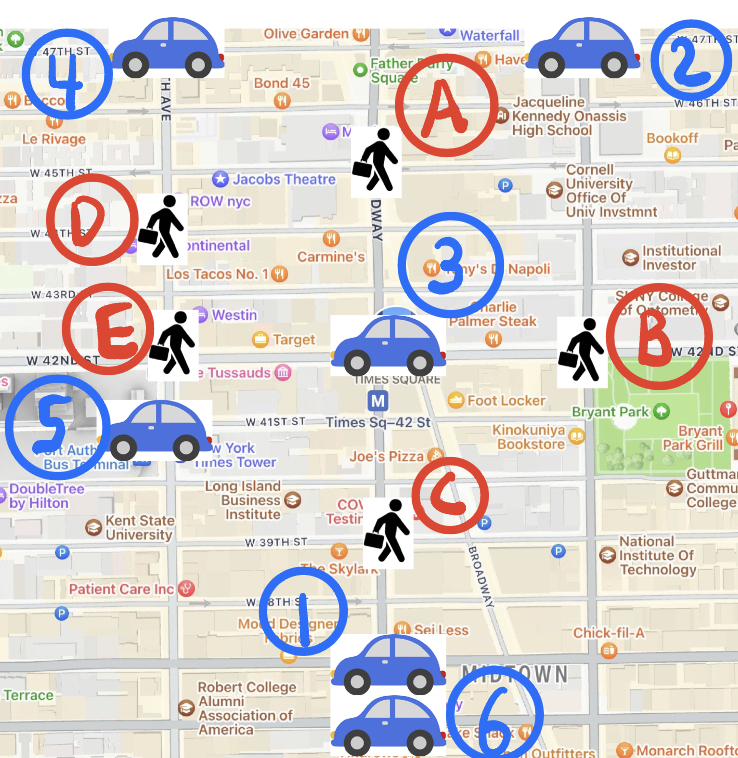
\includegraphics[width=0.87\textwidth]{NYC-map-zoomed-light.jpeg}
        \label{fig:travel_time_graph}
    \end{figure}

    Given a schematic like this, Lyber's goal is to serve as many customers (labeled A--E in the map) as possible, by assigning each one to a driver (labeled 1--6 in the map). For simplicity, each customer and driver is at an intersection, and assume driving between adjacent streets (vertical segment) takes 30 seconds, and driving between adjacent avenues (horizontal segments) takes 1 minute. However, the one twist is that they want to make sure that \textit{no customer is waiting for longer than 2 minutes}.  They also do not want to assign a driver to more than one customer at once, since serving a single customer can take more than 2 minutes.

    \begin{enumerate}
        \item To perform the assignment, they reduce to Maximum Matching in bipartite graphs.  Draw a bipartite graph corresponding to the drivers and customers in the map above.
        \begin{figure}[H]
            \centering
            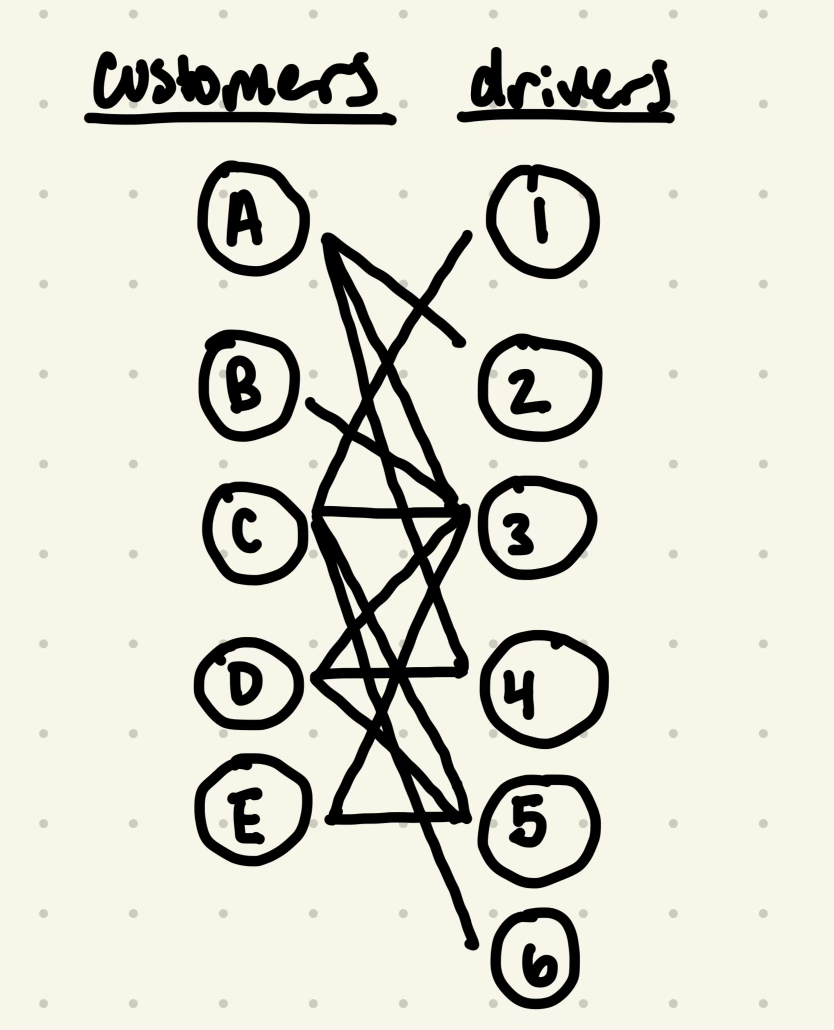
\includegraphics[width=0.2\textwidth]{IMG_0109.png}
            \label{fig:pic1}
        \end{figure}
    
        
        \item The Lyber app first prioritizes customers on Broadway, so they initially assign customer $A$ to driver 3 and customer $C$ to driver 5. Using the algorithm from class, find a \textit{maximum matching} in the bipartite matching graph you've drawn, starting from the initial matching of $A$ to 3 and $C$ to 5. Draw pictures showing the sequence of matchings and augmenting paths you find. (No need to break down the steps of the algorithm to find the augmenting paths.)
        \begin{figure}[H]
            \centering
            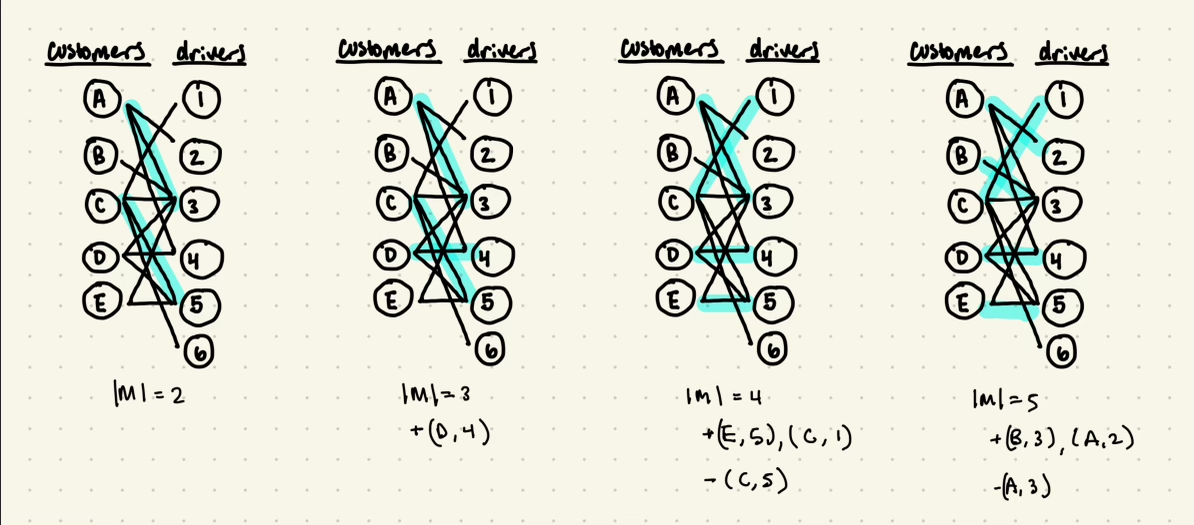
\includegraphics[width=0.87\textwidth]{IMG_0110.png}
            \label{fig:pic2}
        \end{figure}
    \end{enumerate}
    \newpage
    \item (Vertex-Weighted Matching)
        For a graph $G=(V,E)$ and a subset $F\subseteq E$, let $V(F)$ denote the set $\bigcup_{f \in F}f$ of vertices that are an endpoint of at least one edge in $F$.
        \begin{enumerate}
            \item Prove that if $G=(V,E)$ is a graph and $M\subseteq E$ is a matching in $G$, then there is a maximum-size matching $M'$ such that $V(M)\subseteq V(M')$.  (Hint: consider constructing a maximum matching via augmenting paths, but starting with $M_0=M$ rather than $M_0=\emptyset$. What can you say about the $V(M_i)$'s?) \label{part:monotonicity}\\
            
            \textit{Solution. } As per the hint, we construct a maximum matching via augmenting paths, but we'll start with $M_0=M$ rather than $M_0=\emptyset$. 

            By Berge's theorem, while the current matching $M_t$ is not a maximum, there exists some augmenting path with respect to $M_t$ that our algorithm can find. Therefore we can augment our current matching by increasing it at each timestep until we have reached the maximum matching (which can be achieved in finite steps). 

            At any time step $t$, $V\left(M_{t-1}\right) \subseteq V\left(M_t\right)$. This is because when we augment our current matching and increase its size, we do this by flipping which edges of the augmenting path we include in our matching. Notice that when we do this, we keep all the vertices in the original matching, and only encapsulate \emph{more} vertices when we increase the number of edges. Therefore by induction, $V\left(M_0\right) \subseteq V\left(M_1\right) \subseteq \cdots \subseteq V\left(M^\prime \right) \rightarrow V\left(M_0\right) \subseteq V\left(M^\prime \right)$. \\

        \item   In the Embedded EthiCS module, we saw how simply maximizing the {\em size} of a matching may not always be the right objective.  Thus, it is natural to consider weighted versions of the matching problem. Suppose 
        we consider vertex-weighted graphs $G = (V,E,w)$, $w$ is an array specifying a nonnegative vertex weight $w(v)$ for every $v\in V$.  (For example, the weight assigned to a patient might correspond to the number of extra years of life they would gain from a donation.)
          The goal of the {\em vertex-weighted maximum matching problem} is to find a matching $M$ maximizing its {\em total weight} $$w(M) = \sum_{\{u,v\}\in M} (w(u)+w(v)).$$
        (This corresponds to the utilitarian objective discussed in Embedded EthiCS module.)
        Using the part about monotonicity, prove that every graph $G$ has a matching $M^*$ that simultaneously maximizes both total weight and size.  That is, for every matching $M$ in $G$, we have
        both $w(M)\leq w(M^*)$ and $|M|\leq |M^*|$.

        This still leaves the question of whether there efficient algorithms to optimize vertex-weighted matching.  This problem can be reduced to the maximum-flow problem, which is covered in CS1240.\\

        \textit{Solution. } We will show that every graph $G$ has a matching $M^*$ that simultaneously maximizes both total weight and size using contradiction. Suppose that there exists a matching $M^*$ that maximizes total weight, but not total size. But then from part (a), we know there exists a maximum matching $M^{\prime}$ where $V(M^*) \subseteq V\left(M^{\prime}\right)$, so $M^*$ does not maximize total weight, as $V\left(M^{\prime}\right)$ contains a superset of all of the vertices in $M^*$. Therefore by contradiction, every graph $G$ has a matching $M^*$ that simultaneously maximizes both total weight and size.

        \item (optional\footnote{This problem won't make a difference between N, L, R-, and R grades. As this problem is purely extra credit, course staff will deprioritize questions about this problem at office hours and on Ed.}) Show how to reduce matching with the {\em maximin} objective to vertex-weighted matching,\footnote{In lecture, Salil said that he did not know whether there were efficient algorithms to optimize the maximin objective, but afterwards we realized that this reduction allows it to be solved via maximum flow algorithms, as covered in CS1240.}
        and deduce that there is always a matching $M$ that simultaneously maximizes the maximin objective and $|M|$.  For simplicity, you may assume that there are no ties in how well off the patients are prior to treatment.  (Hint: use weights that are powers of 2.)\\

        \textit{Solution. } We could define the maximin objective function as 
        $$
        s(M) = \begin{cases}
            -\infty & \text{if } v_{\min} \text{ is not matched by } M, \\
            \max \{ w(u) : (u, v) \in M \} & \text{otherwise.}
            \end{cases}
        $$
        where $v_{\min }$ is the vertex with the smallest weight and $v_{\min }=\arg \min _{v \in V} w(v)$. To maximize this, either:

        1: $v_{\min }$ is isolated, in which case we can have any matching\\
        2: $v_{\min }$ is connected, so we want the matching to contain the edge that maximizes the weight of the vertex connected to $v_{\min }$. To do this, we can run MaxMatchingAugPaths starting from an initial matching $M_0$ which contains this edge. From part (a), we know this can expand to a maximum matching. \\
        Therefore, there is always a matching $M$ that simultaneously maximizes the maximin objective and $|M|$.
        
        \end{enumerate}

    \item (EthiCS Reflection) Suppose there are two patients in need of an immediate kidney transplant, but only one donor is currently available. The donor’s kidney is compatible with both patients. Patient A starts at 30 QALYs and is expected to live 3 additional QALYs as a result of the transplant. Patient B starts at 45 QALYs, and is expected to live 10 additional QALYs as a result of the transplant. {\em All else being equal}, \textbf{which patient should the kidney go to, and why?} Your response should take the form of a short paragraph (3-4 sentence) reflection. In explaining your ethical reasoning about the case, be sure to draw on at least one concept discussed in class.

    \textit{Note: As with the previous psets, you may include your answer in your PDF submission, but the answer should ultimately go into a separate Gradescope submission form.}

    \item Once you're done with this problem set, please fill out \href{https://forms.gle/4D5u71QSidk4VLoV9}{this survey} so that we can gather students' thoughts on the problem set, and the class in general. It's not required, but we really appreciate all responses!
    
\end{enumerate}

\end{document}